\documentclass{article}
\usepackage[osf,tabular,sfdefault]{biolinum}
\usepackage[scale=.75]{FiraMono}
\usepackage[onehalfspacing]{setspace}
\usepackage{sfmath,amsmath,bm}
\usepackage[marginal]{footmisc}
% shorthands
\usepackage[
  colorlinks,
  linkcolor=blue,
  citecolor=magenta,
]{hyperref}
\usepackage{xspace}
\newcommand{\covid}{\mbox{\textsc{covid-19}}\xspace}
\newcommand{\polymod}{\mbox{\textsc{polymod}}\xspace}
\newcommand{\hreftt}[1]{\href{#1}{\texttt{#1}}}
\setlength{\skip\footins}{\bigskipamount}
\newcommand{\rom}[1]{\textsc{\romannumeral#1})}
% bib
\addbibresource{refs}
% floats
\usepackage{graphicx}
\graphicspath{{fig/}}
\usepackage{booktabs}
\usepackage{subcaption}
\newcommand{\floatfoot}[2][1]{%
  \par\parbox{#1\linewidth}{\footnotesize#2}}

\begin{document}
  \maketitle
  \section{Objective}\label{s:obj}
  Consider a population stratified by into
  $A=11$ age groups ($a$) and $N=510$ neighbourhoods (FSA, $n$).
  %  A proportion $\e_n$ of individuals in FSA $n$ are essential workers.
  We are interested in defining the number of contacts formed between
  all individuals in group $na$ and all individuals in group $n'a'$,
  which we denote $X_{nan'a'}$.
  Then, we will use a pre-determined assignment FSAs into $G=10$ groups (deciles, $g$)
  to aggregate the FSA dimensions and obtain $X_{gag'a'}$.
  \section{Approach}\label{s:methods}
  \subsection{Data}\label{ss:data}
  We know the sizes of populations in each FSA $n$, stratified by age groups $a$,
  which we denote $P_{na}$.
  Anonymous cell phone mobility data from Ontario has also been used to estimate
  the average proportion of individuals living in FSA $n$ who travel to FSA $n'$ per day
  for at least one hour, which we denote $B_{nn'}$.
  These proportions are aggregated into groups $gg'$ and shown in Figure~\ref{fig:mobility}.
  Finally, the \textsc{polymod} study estimates the average numbers of contacts per person per day
  between age groups $a$ and $a'$, stratified by the following types ($y$) of contacts:
  \emph{home}, \emph{work}, \emph{school}, \emph{transport}, \emph{leisure}, \emph{other};
  these data are denoted $C_{aa'y}$ and are illustrated in Figure~\ref{fig:polymod}.
  \subsection{Contact Rates}\label{ss:contacts}
  The total number of type $y$ contacts per individual in age group $a$ per day
  in the \textsc{polymod} study can be obtained by summing across the ``other'' age groups $a'$:
  \begin{equation}
    C_{ay} = \sum_{a'} C_{aa'y}
  \end{equation}
  We assume these contact rates apply to our population.
  Thus, the total number of type $y$ contacts made available by age $a$ individuals in FSA $n$ is:
  \begin{equation}
    Q_{nay} = P_{na} C_{ay}
    \label{eq:Qnay}
  \end{equation}
  These contacts can be formed with three potential mixing pools:
  (a) others met while travelling to another FSA $n'$;
  (b) others met who travelled to this FSA $n$; and
  (c) others within this FSA $n$ only.
  For a given contact type $y$, we assume that a proportion $h_y$
  of those contacts are be formed with pool~(c).
  We further assume that the remaining contacts $(1-h_y)$ are formed
  with pools (a,b) in proportion to population mobility.
  That is the proportion who are mobile form these contacts with (a),
  and the proportion who are not form these contacts with (b).
  Let $B_n = \sum_{B_{nn'}}$ be the total mobile proportion.%
  \footnote{The current implementation in code introduces another parameter
    to control the total mobile population directly.}
  Then $Q_{nay}$ are distributed amongst the mixing pools as:
  \begin{equation}
    Q_{nay} \sim
    \begin{cases}
      B_n (1-h_y)     & \textrm{(a) other traveller pools} \\
      (1-B_n) (1-h_y) & \textrm{(b) local traveller pool} \\
      h_y             & \textrm{(c) local non-traveller pool} \\
    \end{cases}
  \end{equation}
  Now consider the traveller pool in FSA $n^*$,
  comprising (a) contacts from other FSAs and (b) contacts from this FSA.
  The total number of type $y$ contacts made available to the pool
  by age~$a$ individuals from FSA~$n$ is
  (where $1_{x=y}$ denotes $1$ if $x=y$ else $0$):
  \begin{equation}
    Q^{n^*}_{nay} = Q_{nay} (1-h_y) \left(B_{nn^*} + 1_{n=n^*}(1-B_n)\right)
  \end{equation}
  Thus, the total number of contacts made available to the pool is:
  \begin{equation}
    T_{n^*y} = \sum_{na} Q^{n^*}_{nay}
  \end{equation}
  We assume that contacts form randomly with respect to home FSA $n$,
  but the \textsc{polymod} data suggest that contacts do not form randomly with respect to age.
  We cannot use the \textsc{polymod} contact matrices directly,
  since these depend on the distribution of age groups from the \textsc{polymod} study,
  and thus would not balance given the different age distributions between FSAs.
  However, we can assume a parametric form for age mixing, such as:
  \begin{equation}
    Q'_{aa'y} = Q_{ay} \left( (1 - \epsilon_y) \pi_{a'y} + (\epsilon_y) 1_{a=a'} \right),\quad
    \pi_{a'y} = \frac{Q_{a'y}}{\sum_{a'}Q_{a'y}}
    \label{eq:eps}
  \end{equation}
  where $\epsilon_y \in [0,1]$ denotes the degree of assortative (like-with-like) mixing by age groups.
  The value of $\epsilon_y$ can be estimated based on \textsc{polymod} data,
  by minimizing the difference between the empiric $Q_{aa'y}$ and the parametric approximation $Q'_{aa'y}$,
  using $Q_{ay} \approx C_{ay}$ (no population weighting).
  A good measure of ``difference'' is the Kullback-Leibler Divergence:%
  \footnote{The contact matrices $C_{aa'y}$ and $C'_{aa'y}$ are not strictly probability distributions
    because they sum to more than one.
    We could normalize $C_{aa'y}$ and $C'_{aa'y}$ by $\sum_a C_{ay}$ to compute a ``proper'' KL-Divergence.
    However, as can be seen in Eq~(\ref{eq:DKL}), this constant will not affect the minimization.}
  \begin{equation}
    D_{\textrm{KL}}(Q_{aa'y} \mid\mid Q'_{aa'y}) = \sum_{aa'} Q_{aa'y} \log{\left(\frac{Q_{aa'y}}{Q'_{aa'y}}\right)}
    \label{eq:DKL}
  \end{equation}
  The estimated $\epsilon_y$ using this approach are given in Figure~\ref{fig:polymod}.
  Returning to the traveller pool in FSA $n^*$,
  the total number of type $y$ contacts formed between people aged $a$ from FSA $n$
  with people aged $a'$ from FSA $n'$ is then given by:
  \begin{equation}
    X^{n^*}_{nan'a'y} =
      (1-\epsilon_y) \pi^{n^*}_{nan'a'y} +
        (\epsilon_y) 1_{a=a'} \sum_{a'} \pi^{n^*}_{nan'a'y}
    \thinspace,\quad
    \pi^{n^*}_{nan'a'y} = \frac{Q^{n^*}_{nay} Q^{n^*}_{n'a'y}}{T_{n^*y}}
  \end{equation}
  The total number of contacts formed between FSA $n$ and FSA $n'$ is then
  the sum across all traveller pools, including those corresponding to $n=n^*$ and $n'=n^*$,
  plus the local contacts from case (c):
  \begin{equation}
    X_{nan'a'y} = \sum_{n^*} X^{n^*}_{nan'a'y} + 1_{n=n'}\left( (1-h_y) \sum_{n'} X^{n^*}_{nan'a'y} \right)
  \end{equation}
  \subsection{Caveats}\label{ss:caveats}
  \begin{itemize}
    \item We introduced a 6 free parameters in $h_y$, representing
          the proportion of type $y$ contacts that are formed with the local non-traveller pool.
          However, some values of $h_y$ can likely be fixed, such as
          $h_1 = 1$: no \emph{home} contacts formed with the traveller pool, etc.
    \item We assume that travelling individuals only form contacts in one destination.
          However, due to the large numbers involved,
          this assumption won't likely have any influence on the results.
    \item We have not considered differences in contact numbers by FSA $n$,
          for example, due to different types of employment or housing.
          However, this could be added to $Q_{nay}$ in Eq.~(\ref{eq:Qnay}).
  \end{itemize}
  \section{Results}\label{s:results}
  \paragraph{Note}
  In Section~\ref{s:methods} we described the methodology in relation to $N=510$ FSAs.
  However, as noted in Section~\ref{s:obj}, we eventually intended to aggregate the mixing matrices
  to reflect $G=10$ groupings of FSAs.
  Since the mobility data currently available are based on these groupings ($g$),
  the results below are for the groupings.
  When analyzing groups $g$ instead of FSAs $n$,
  the methodology above can be repeated exactly using $n \rightarrow g$,
  $Q_{nay} \rightarrow Q_{gay}$, and $B_{nn'} \rightarrow B_{gg'}$,
  which can be obtained as suggested in v.1 of this report
  (where $S_g$ is the set of $n$ assigned to group $g$):
  \begin{equation}
    Q_{gay} = \sum_{n \in S_g} Q_{nay},\quad
    B_{gg'} = \sum_{n \in S_g} \sum_{n' \in S_{g'}} B_{nn'}
  \end{equation}
  \par
  The estimated values of $\epsilon_y$ corresponding to
  the degree of assortative age mixing by contact type were:
  \emph{home}: 0.09, \emph{work}: 0.03, \emph{school}: 0.22, \emph{transport}: 0.12, \emph{leisure}: 0.13, \emph{other}: 0.06.
  Figure~\ref{fig:polymod} compares the original \textsc{polymod} contact data with
  the values approximated by the parametric equation (\ref{eq:eps}).
  \par
  Figure~\ref{fig:Xggy} illustrates the total number of contacts (millions)
  predicted between deciles, stratified by contact type,
  using $h_y = [1,0,1,0,\frac{1}{2},\frac{1}{2}]$.%
  \footnote{And also assuming 50\% population mobility}
  We verified that $\sum_{g'a'} {X_{gag'a'y}} = Q_{gay}$ for all contact types $y$.
  When $h_y = 0$ (e.g. \emph{home} contacts), the contact matrix has no off-diagonal elements.
  However, even for $h_y = 1$ (e.g. \emph{work} contacts),
  the contact matrix is still dominated by the diagonal
  due to the tendency for individuals to move between FSA in the same decile
  (Figure~\ref{fig:mobility}),
  and the larger size of the non-mobile population (locals) in the local traveller pool.
  The proportions of all contacts formed within the same decile across the various contact types was:
  \emph{home}: 1.00, \emph{work}: 0.33, \emph{school}: 1.00, \emph{transport}: 0.33, \emph{leisure}: 0.67, \emph{other}: 0.67;
  and 0.72 overall.
  To improve readability, Figure~\ref{fig:Xggy} therefore also shows the number of contacts
  in the off-diagonal elements alone.
  Finally, Figure~\ref{fig:Xgg} similarly illustrates the total number of contacts (millions)
  predicted between deciles, after aggregating over contact types.
  \clearpage\newgeometry{margin=2cm}
  \begin{lswide}
    \begin{figure}[H]
      \centering
      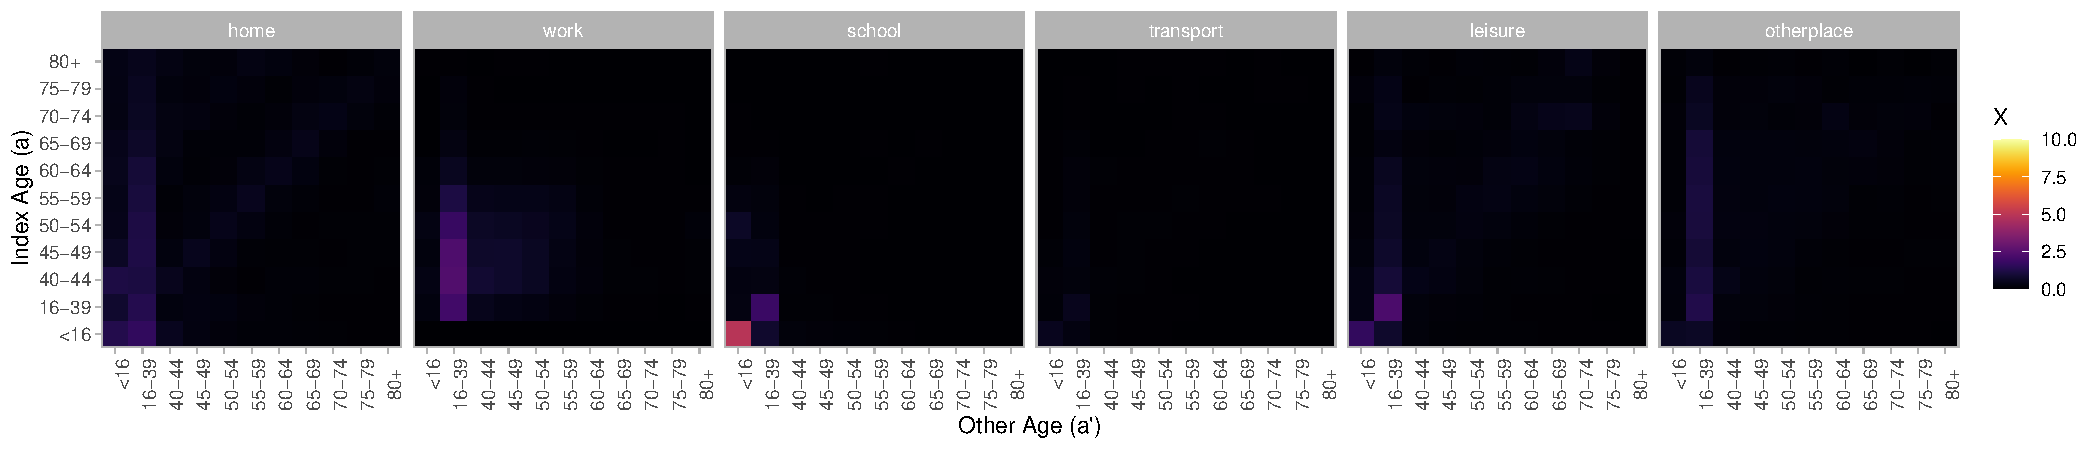
\includegraphics[height=0.3\textheight]{polymod.pdf}\subfig{A}
      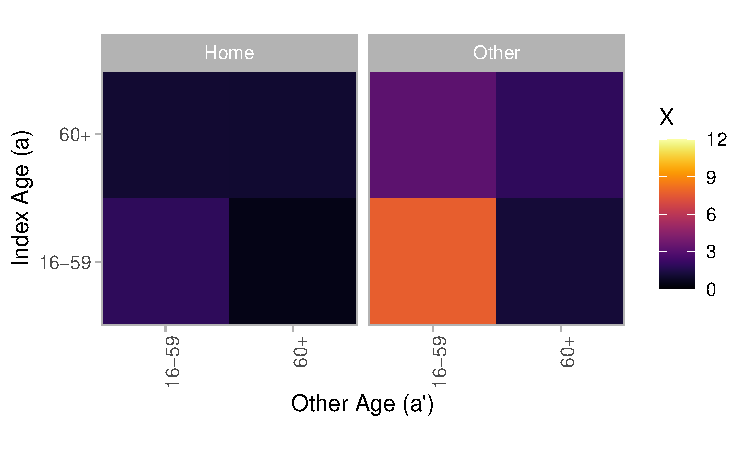
\includegraphics[height=0.3\textheight]{polymod-eps.pdf}\subfig{B}
      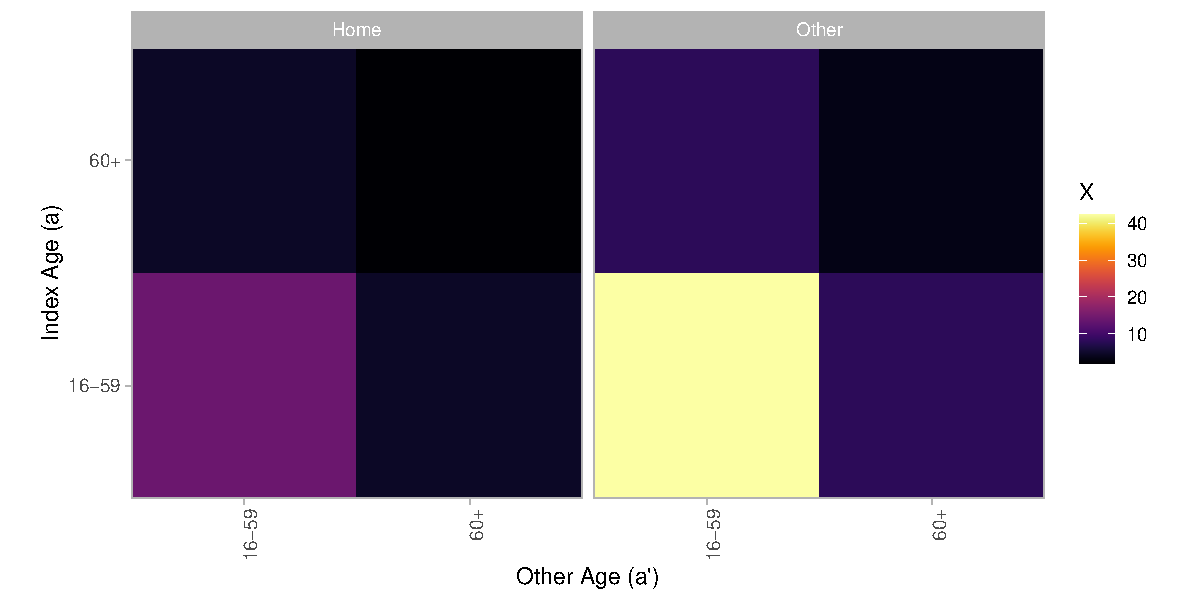
\includegraphics[height=0.3\textheight]{Xaay.pdf}\subfig{C}
      \caption{Average number and types of contacts between individuals of various age groups per day.
        A:~original \textsc{polymod} data;
        B:~parametric approximation of \textsc{polymod} data;
        C:~total contacts modelled in Ontario in conjunction with mobility data.}
      \label{fig:polymod}
    \end{figure}
  \end{lswide}
  \begin{lswide}
    \begin{figure}[H]
      \centering
      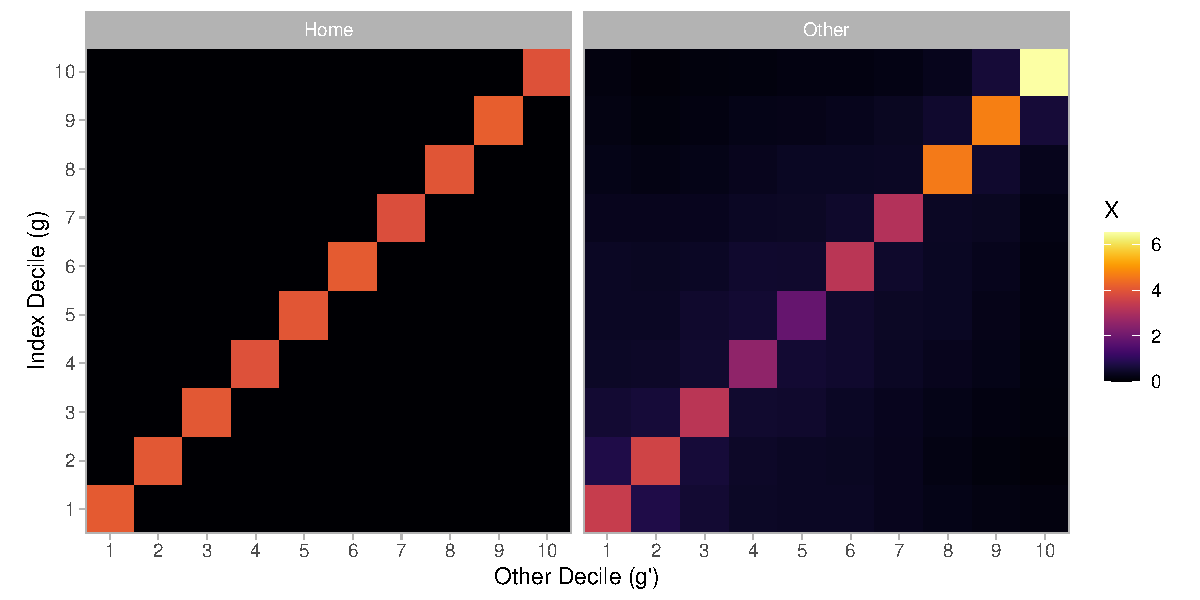
\includegraphics[height=0.3\textheight]{Xggy.pdf}
      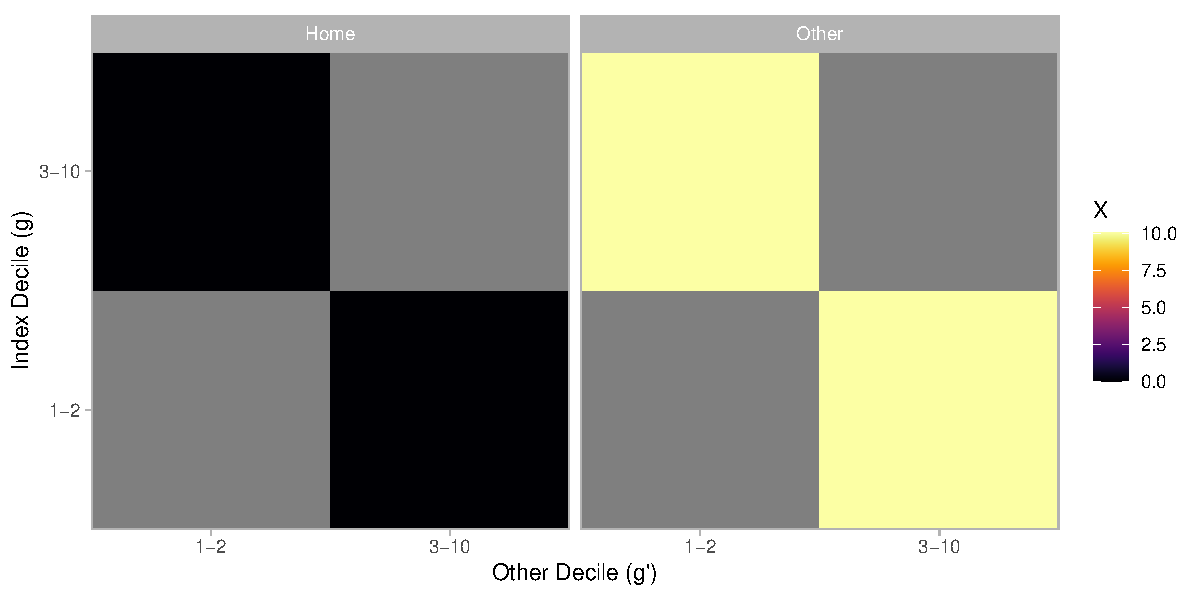
\includegraphics[height=0.3\textheight]{Xggy-o.pdf}
      \caption{Total number and types of contacts formed between deciles (millions);
        raw values (top) and after removing the dominant diagonal (bottom)}
      \label{fig:Xggy}
    \end{figure}
  \end{lswide}
  \begin{figure}[H]
    \centering
    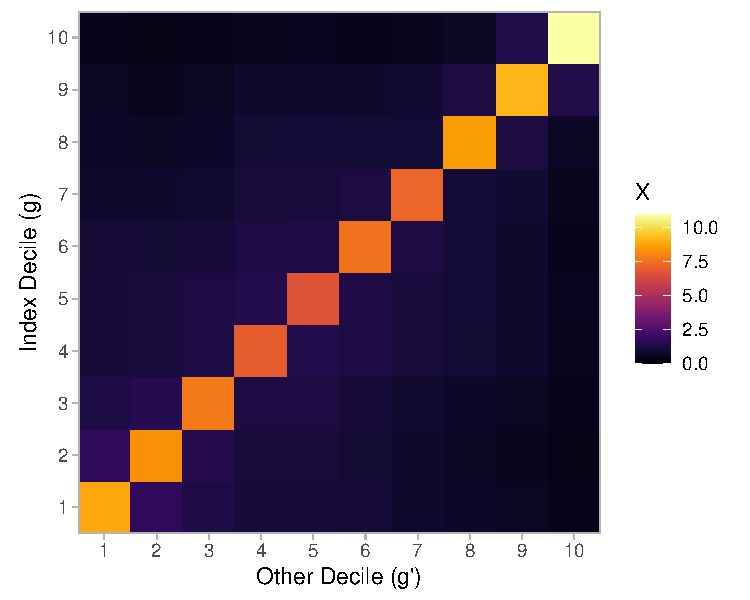
\includegraphics[width=.4\linewidth]{Xgg.pdf}
    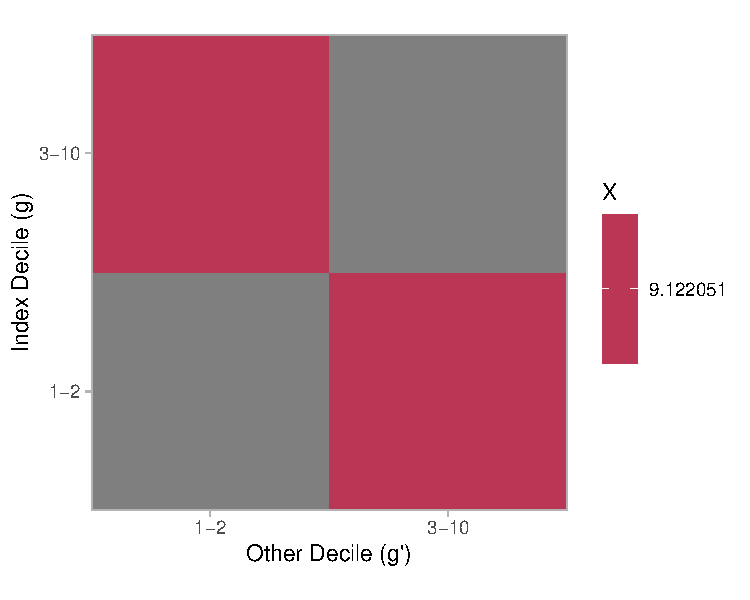
\includegraphics[width=.4\linewidth]{Xgg-o.pdf}
    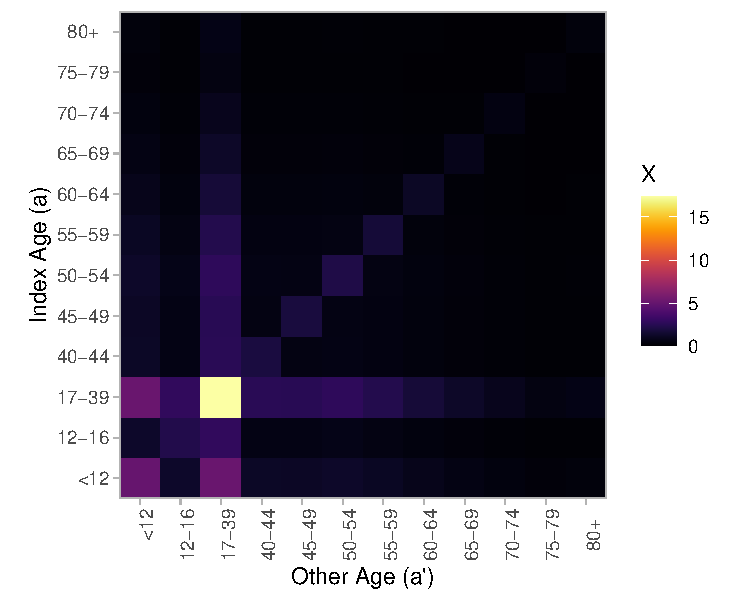
\includegraphics[width=.4\linewidth]{Xaa.pdf}
    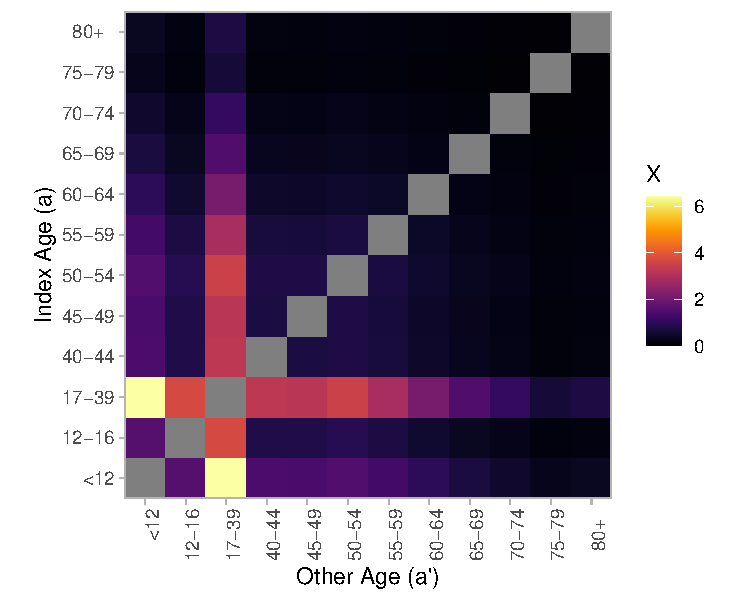
\includegraphics[width=.4\linewidth]{Xaa-o.pdf}
    \caption{Total number of contacts (millions) formed between deciles (top) and age groups (bottom);
      complete values (left) and after removing the dominant diagonals (right)}
    \label{fig:Xgg}
  \end{figure}
  \begin{figure}[H]
    \centering
    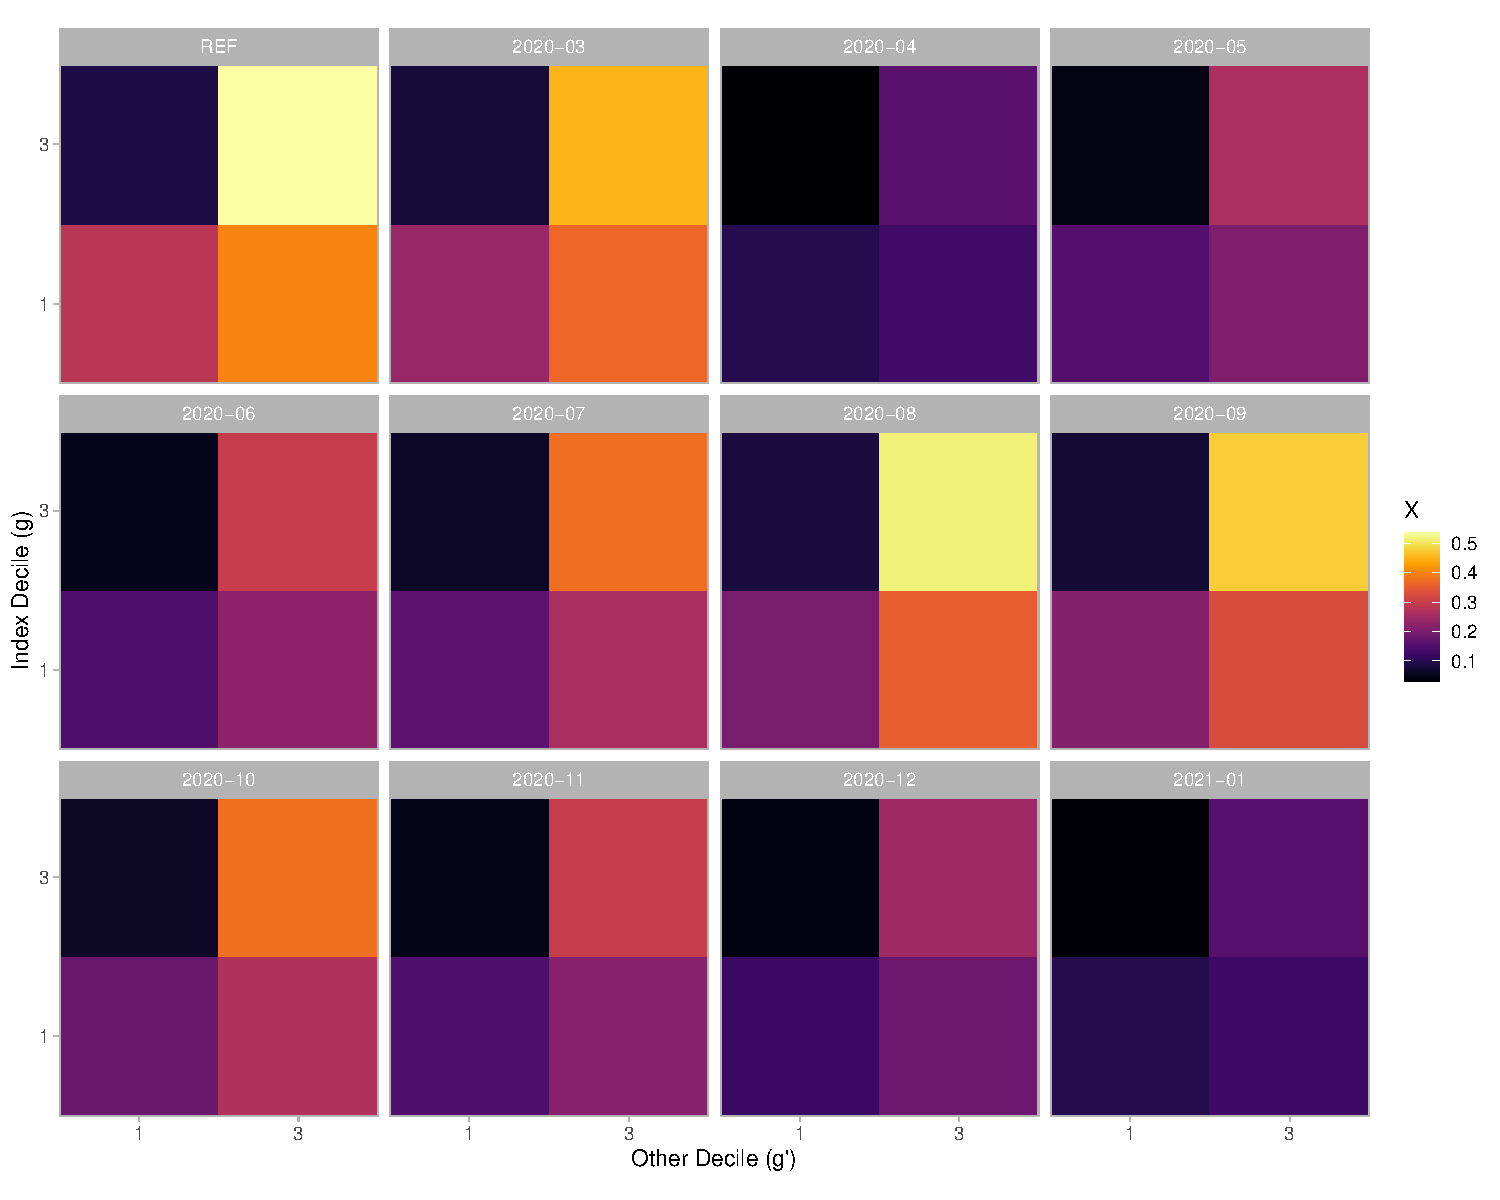
\includegraphics[width=.4\linewidth]{mobility.pdf}
    \caption{Cell phone mobility data:
      proportion of individuals residing in ``index decile'' who travelled to ``other decile''
      for at least one hour per day}
    \label{fig:mobility}
  \end{figure}
\end{document}